\begin{figure}[tb]
    \centering
    \begin{minipage}[t]{0.48\textwidth}
        \centering
        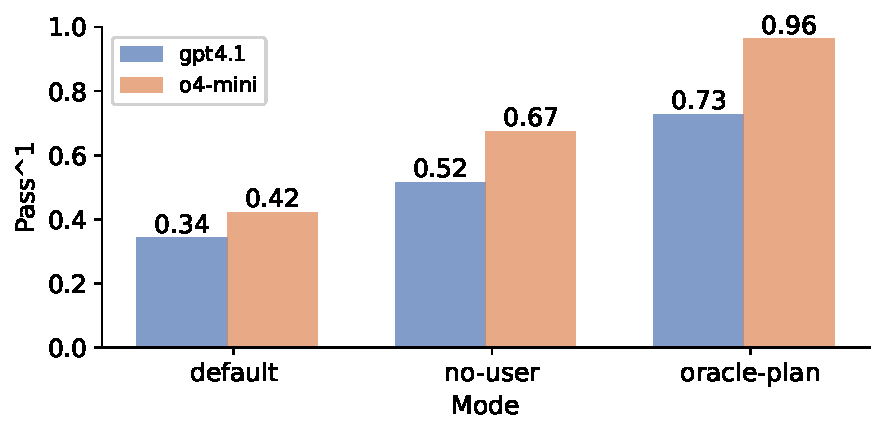
\includegraphics[width=\linewidth]{figures/results/pass_one_metrics_telecom_bar.pdf}
    \end{minipage}
    \hfill
    \begin{minipage}[t]{0.48\textwidth}
        \centering
        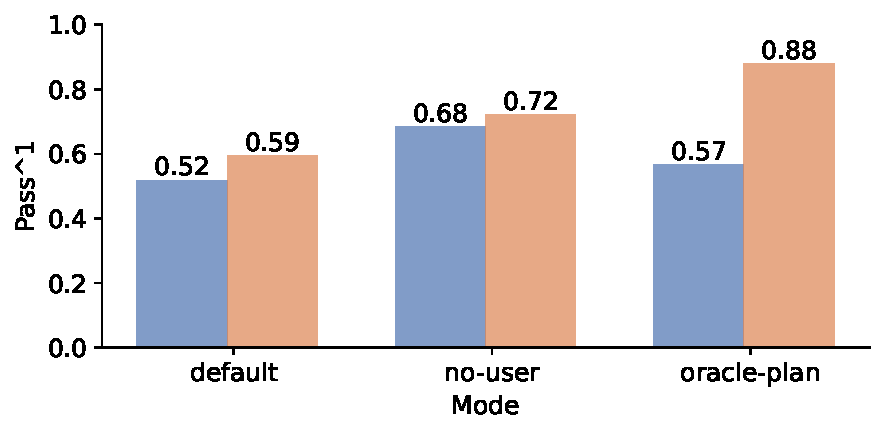
\includegraphics[width=\linewidth]{figures/results/pass_one_metrics_telecom-workflow_bar.pdf}
        \vspace{-1.5em}
    \end{minipage}
    \caption{\basemode 사용자 시뮬레이션을 사용했을 때, 서로 다른 운영 모드(\basemode, \solomode, \gtmode)에 걸친 Telecom 도메인의 \passone 지표. \textbf{왼쪽}: 원래 정책. \textbf{오른쪽}: workflow 기반 정책. 이 그림은 추론 부하와 분산 제어가 에이전트 성능에 미치는 영향을 보여 준다.}
    \label{fig:telecom_avg_bar}
\end{figure}
